\section{\Multidispatch{} Linearizability}
\label{sec:mdl}

In this section, we first define \multidispatch{} linearizability.
We then show how applications built atop an \MDL{} system appear
to behave identically (as far as users can tell) to the same application interacting
with a comparable \SDL{} system. Finally, we discuss existing implementations
of \MDL{} for single-shard systems and why they do not trivially extend to more
shards.

We leverage the formalism used in Helt et al.~\cite{helt2021rss}.

\subsection{Users, Applications, \& Executions}
\label{sec:mdl:applications}

We model a distributed \textit{application} as a collection of $n$
\textit{processes}. Processes are state machines~\cite{lynch1987ioa,lynch1996da}
that implement application logic by performing local computation, exchanging
messages, and invoking operations on systems.

An application's processes define a prefix-closed set of \textit{executions},
which are sequences $s_0,\pi_1,s_1,\ldots$ of alternating \textit{states} and
\textit{actions}, starting and ending with a state. An application state
contains the state of each process---it is an $n$-length vector of process
states. As part of a process's state, we assume it has access to a local
clock, which it can use to set local timers, but the clock makes no guarantees
about its drift or skew relative to those at other processes.

Each action is a step taken by exactly one process and is one of three types:
\textit{internal}, \textit{input}, or \textit{output}. Internal actions model
local computation. Processes use input and output actions to interact with other
processes (e.g., receiving and replying to a remote procedure call) and their
environment (e.g., responding to a user gesture). As we will describe in the
following section, a subset of the input and output actions are
\textit{invocations} and \textit{responses}, respectively, which are used to
interact with systems.

Processes can also exchange messages with one another via unidirectional
channels. To send a message to process $P_j$, $P_i$ uses two actions: first,
$P_i$ uses an output action $\sendto_{ij}(m)$ and later, an input action
$\sent_{ij}$ occurs, indicating $m$'s transmission on the network. Similarly, to receive a
message from $P_i$, $P_j$ first uses an output action $\request_{ij}$ and later,
an input action $\receive_{ij}(m)$ occurs, indicating the receipt of $m$.

Given an execution $\alpha$, we will often refer to an individual process's
\textit{sub-execution}, denoted $\alpha|P_i$. $\alpha|P_i$ comprises
only $P_i$'s actions and the $i$th component of each state in $\alpha$.

\noindentparagraph{Well-formed.} An execution is \textit{well-formed} if it
satisfies the following: (1) Messages are sent before they are received; (2) A
process has at most one (total) outstanding invocation (at a system)
or $\request_{ij}$ (at a channel); and (3) Processes do not take output steps while
waiting for a response from a system. We henceforth only consider well-formed executions.

TODO: Update definition of well-formed.
% A \textit{process sub-history} $H|P$ is the subsequence of all invocations and responses
% in $H$ invoked or received by the application process $P$. To define \MDL{}, we relax the
% assumption made by Herlihy et al.~\cite{herlihy1990linearizability} that process sub-histories
% (i.e., their interactions with the system) are sequential. Instead, we say a history $H$
% is \textit{well-formed} if the following hold for each process sub-history $H|P$:
% (1) $H|P$ starts with an invocation, and (2) for each operation $o$, if $\res(o)$ is in $H$,
% it follows (not necessarily immediately) $\inv(o)$. We consider only well-formed histories.

TODO: Add users.

TODO: Define $||$.
% Given a history $H$, $H||P$ is a \textit{sequentialization} of $H|P$. $H||P$ is
% found by, for each complete operation $o$ in $H|P$, shifting $\res(o)$ left (earlier) in $H|P$
% until it immediately follows $\inv(o)$. Note that if $H|P$ is sequential, then $H|P = H||P$.

\subsection{Systems}
\label{sec:mdl:systems}

Databases, message queues, and other back-end \textit{systems} that application
processes interact with are defined by their \textit{operations} and a
\textit{specification}~\cite{herlihy1990linearizability,lynch1996da}. An
\textit{operation} comprises pairs of \textit{invocations}, specifying the
operations and their arguments, and matching \textit{responses}, containing
return values. The specification is a prefix-closed set of sequences of
invocation-response pairs defining the system's correct behavior in the absence
of concurrency. A sequence $S$ in specification $\spec$ defines a total order
over its operations, denoted $<_S$.

\subsection{Definition}
\label{sec:mdl:def}

We are now ready to define two (last) preliminaries and then our new consistency model.

\noindentparagraph{Complete operations.} Given an execution $\alpha$, we say an
operation is \textit{complete} if its invocation has a matching response in
$\alpha$. We denote $\complete(\alpha)$ as the maximal subsequence of $\alpha$
comprising only complete operations~\cite{herlihy1990linearizability}.

\noindentparagraph{Real-time order.} Two actions in an execution $\alpha$ are
ordered in real
time~\cite{herlihy1990linearizability}, denoted
$\pi_1 \rt_\alpha \pi_2$, if and only if $\pi_1$ is a response, $\pi_2$ is an
invocation, and $\pi_1$ precedes $\pi_2$ in $\alpha$.

\noindentparagraph{\Multidispatch{} Linearizability.} Let $\mathcal{O}$ be the
set of all operations. An execution $\alpha_1$ satisfies \textit{\MDL{}} if it
can be extended to $\alpha_2$ by adding zero or more responses such that there
exists a sequence $S \in \spec$ where (1) for all $P$,
$S|P = \complete(\alpha_2)||P$; and (2) for all pairs of operations
$o_1,o_2 \in \mathcal{O}$, $o_1 \rt_{\alpha_1} o_2 \implies o_1 <_S o_2$.

\subsubsection{Suffix-Closed Failures}
\label{sec:mdl:def:failures}

\MDL{}'s definition has an important implication for system designers.
In systems where operations can fail (even temporarily before being retried), the effects
of an operation cannot be exposed to other processes until all of its predecessors are
guaranteed to succeed. Doing so would violate the intuitively correct behavior of most
systems, and formally, this would result in $S|P \neq \complete(\alpha_2)||P$ for all legal
sequential histories $S \in \spec$. We refer to this property as
\textit{suffix-closed failure semantics}.

In an \MDL{} system, suffix-closed failures must be guaranteed even in the
face of concurrent operations from the same process, which in practice may to
objects on different shards. As we will see in Section~\ref{sec:mdl:zookeeper},
guaranteeing suffix-closed failures is one way in which existing systems fail
to correctly implement \multidispatch{} linearizability.  

\subsection{External Equivalence}
\label{sec:mdl:equivalence}

In this section, we show how we can transform an application that interacts with
a (\singledispatch{}) linearizable system to take advantage of a comparable
\multidispatch{} system. Importantly, our transformation will ensure that the new
application appears to behave identically to the original application (as far as
the users can tell).

We begin by defining several preliminaries, including the transformation. We then
present a condensed form of the proof that the transformation preserves external
equivalence. For ease of exposition, we focus on the actions within an
execution and assume states can be modified and reordered as needed.

\noindentparagraph{Definition.} Two executions $\alpha$ and $\beta$ are
\textit{externally equivalent} if $\alpha|U = \beta|U$. Intuitively,
externally equivalent executions are indistinguishable to users.

\begin{thm}
Let $A$ be an application designed to interact with a linearizable system,
and let $A^\prime = \transform(A)$ be the transformed application. Suppose
$\alpha^\prime$ is an execution of $U \times C \times A^\prime$ that satisfies
\MDL{}. Then there is an externally equivalent execution $\beta$
of $U \times C \times A$ that satisfies \SDL{}.
\end{thm}

\begin{proof}
The proof proceeds in steps: First, we create an execution $\alpha$ from
$\alpha^\prime$ by essentially undoing the parallelizing transformation in
each process's sub-execution. Second, we produce $\beta$ by fixing the order
of actions across processes to ensure $\beta$ is well-formed and satisfies \SDL{}.

By the assumption that $A$ is well-formed and rules 4 through 7 of $\transform$,
each $\alpha^\prime | P_i$ comprises sub-sequences of local and
system-facing actions separated by non-system-facing external actions.
Further, by rule 5 of $\transform$, the order of the non-system-facing external
actions in each $\alpha^\prime | P_i$ respects the program order of the
original application $A$. 

We first reorder the actions in each sub-sequence of each $\alpha^\prime | P_i$
to place the local and system-facing actions such that they respect $A$'s program
order. More precisely, for each $\alpha^\prime | P_i$ and for each action $\pi$
starting with the right-most, shift $\pi$ left in $\alpha^\prime$ until it precedes
all other actions $\pi^\prime$ in $\alpha^\prime | P_i$ such that $A$'s program
order requires that $\pi$ precedes $\pi^\prime$. Let $\alpha^\prime$ be the
resulting execution.

By the observation about each $\alpha^\prime | P_i$ above, the order of
non-system-facing external actions in $\alpha$ respects $A$'s program order
(because $A^\prime$'s is identical). Further, each $\alpha | P_i$ now
issues its operations sequentially (since $A$'s program order mandates
that operations are issued sequentially).

The execution $\alpha$, however, may not satisfy linearizability. We now remedy this
and produce the needed $\beta$. To do so, first recall that by assumption the original 
$\alpha^\prime$ satisfied \MDL{}, so let $S$ be a total order over the operations
in $\alpha^\prime$ as guaranteed by \MDL{}.

We next let $\caused_{\alpha}$ be the set of the following pairs of actions
$(\pi_i, \pi_j)$ in $\alpha$:
\begin{enumerate}
    \item $\mathbf{<_M}$\textbf{:} $\pi_i$ is a send-to action for some message $M$
    (between two users, from a user to a process, a process to a user,
    or between two processes) and $\pi_j$ is its corresponding receive-from action,
    \item $\mathbf{<_{P_i}}$\textbf{:} $\pi_i$ precedes $\pi_j$ in some $\alpha | P_i$,
    \item $\mathbf{<_U}$\textbf{:} $\pi_i$ precedes $\pi_j$ in $\alpha | U$,
    \item $\mathbf{<_S}$\textbf{:} For each adjacent pair of operations $o_k$, $o_{k+1}$
    in $S$, $\pi_i$ is $o_k$'s response action and $\pi_j$ is $o_{k+1}$'s invocation action, or
    \item \textbf{Transitivity:} there exists some action $\pi_k$ such that $(\pi_i, \pi_k)$
    and $(\pi_k, \pi_j)$ are in $\caused_{\alpha^\prime}$.
\end{enumerate}

We posit $\caused_{\alpha}$ defines an irreflexive partial order over the actions
in $\alpha$. Clearly it is irreflexive; we now prove it is acyclic and transitive.

For sake of contradiction, assume $\caused_{\alpha}$ contains a cycle, and
let $\pi_1 \caused_{\alpha} \pi_2 \caused_{\alpha} \ldots \caused_{\alpha} \pi_1$
be a shortest cycles that does not include any transitive edges.

We first prove several important properties of the cycle.

\noindentparagraph{Property 1.} The cycle contains at least two actions.
This follows from the definitions of $<_M$, $<_{P_i}$, $<_U$, and $<_S$.

\noindentparagraph{Property 2.} The cycle does not contain two consecutive
$<_{P_i}$ edges or two consecutive $<_U$ edges. Otherwise, a shorted cycle
exists since $<_{P_i}$ and $<_U$ are transitive.

\noindentparagraph{Property 3.} The cycle does not contain two consecutive
$<_M$ edges or two consecutive $<_S$. This follows from the definitions of
$<_M$ and $<_S$.

In the remainder of the proof, we will leverage the following lemma. For
sake of brevity, however, we omit its proof.

\begin{lem}
    Let $\pi_1 \caused_{\alpha} \ldots \caused_{\alpha} \pi_n$
    be a sequence of $n$ actions connected any of $<_M$, $<_{P_i}$, $<_U$,
    and $<_S$ edges, and further assume $\pi_1$ is a receive-from action
    and $\pi_n$ is a send-to action. Then $\pi_1$ precedes $\pi_n$ in $\alpha$.
    \label{lem:helper2}
\end{lem}

We now conclude the proof. We proceed by cases:

First, assume the cycle contains at least one $<_M$ edge. Then the cycle can be written as
$\pi_1 <_M1 \pi_2 \caused_{\alpha} \ldots \caused_{\alpha} \pi_n \caused_{\alpha} \pi_1$ 
by re-indexing the actions as needed. By the assumption that $\alpha^\prime$ is well-formed,
the fact that $\alpha$ preserved the order of $\alpha^\prime$'s non-system-facing actions,
and the definition of $\pi_1 <_M \pi_2$, it is clear that $\pi_1$ precedes $\pi_2$ in $\alpha$.

But the remainder of the cycle
$\pi_2 \caused_{\alpha} \ldots \caused_{\alpha} \pi_1$
is a sequence of actions connected by $<_M$, $<_{P_i}$, $<_U$, and $<_S$ edges
starting with a receive-from action ($\pi_2$) and ending with a send-to action
($\pi_1$). Thus, by Lemma~\ref{lem:helper2}, $\pi_2$ precedes $\pi_1$ in $\alpha$,
a contradiction.

Now assume the cycle does not contain any $<_M$ edges. Since there are no messages in
the cycle, there are two sub-cases: the cycle comprises either only $<_U$ edges or
(by Properties 2 and 3) alternating $<_{P_i}$ and $<_S$ edges .

In the former case, a cycle contradicts the definition of $<_U$, so we turn to the latter.
Note that all $P_i$ in the $<_{P_i}$ must be distinct, otherwise a shorter cycle must exist.
Since they alternate with $<_S$ edges, for each $\pi_i <_{P_i} \pi_{i+1}$, we know 
$\pi_i$ is an invocation and $\pi_{i+1}$ is a response.

By definition of $<_{P_i}$, $\pi_i$ precedes $\pi_{i+1}$ in $\alpha | P_i$.
Further, since each process’s system interactions occur sequentially in $\alpha$,
so $\pi_{i}$ must also precede $\pi_{i+1}$'s corresponding invocation.
Since the transformation between $A$ and $A^\prime$ preserves each process’s
invocation order (and so MDL does), this implies $\op(\pi_{i})$ is ordered in $S$
before $\op(\pi_{i+1})$.

As a result, for each $\pi_i <_{P_i} \pi_{i+1}$ in our cycle, we can replace with
a sequence of $<_{P_i}$ and $<_S$ edges that includes the invocations and responses
of all operations in $S$ between $\op(\pi_i)$ and $\op(\pi_{i+1})$ (if any).
This (no longer shortest) cycle implies there is a cycle over operations in $S$.
But this contradicts the definition of \MDL{}, which guarantees a total order.
Thus, $\caused_{\alpha^\prime}$ is acyclic. Combined with the definitions of
$<_M$, $<_{P_i}$, $<_U$, and $<_S$, this also shows it is irreflexive.

Let $\beta$ be a topological sort of $\caused_{\alpha}$ on the actions in
$\alpha$. To conclude the proof, we show $\beta$ is well-formed,
satisfies linearizability, and is externally equivalent to $\alpha^\prime$.

The fact that $\beta$ is well-formed follows from the definition of
$\caused_{\alpha}$. It preserves the order of actions in $U$,
which were unaltered in the transformation from $\alpha^\prime$ to $\alpha$.
Similarly, it preserves the order of each message's send-to and receive-from actions,
and their order was also unaltered in producing $\alpha$. Finally, the original
transformation to $\alpha$ placed the actions of each $\alpha | P_i$ in
the order dictated by $A$'s program order, and this was preserved by
$\caused_{\alpha}$ in producing $\beta$.

By the initial reordering to produce $\alpha$ and the definition of
$\caused_{\alpha}$, the operations across all processes in $\beta$
are sequential in the order defined by $S$. Since $S$ defined a
total order over all operations, $\beta$ thus satisfies linearizability.

Finally, since the initial transformation from $\alpha^\prime$ to $\alpha$
did not alter the order of actions in $U$, clearly $\alpha^\prime | U = \alpha | U$.
Then by the definition of $\caused_{\alpha}$, $\alpha | U = \beta | U$.
$\beta$ is thus externally equivalent to $\alpha$.
\end{proof}

\subsection{\MDL{} Beyond One Shard}
\label{sec:mdl:zookeeper}

In this section, we discuss Zookeeper and its implementation of \SDL{}.
We also show how such an approach does not extend to multiple shards.

\begin{figure}[!htb]
    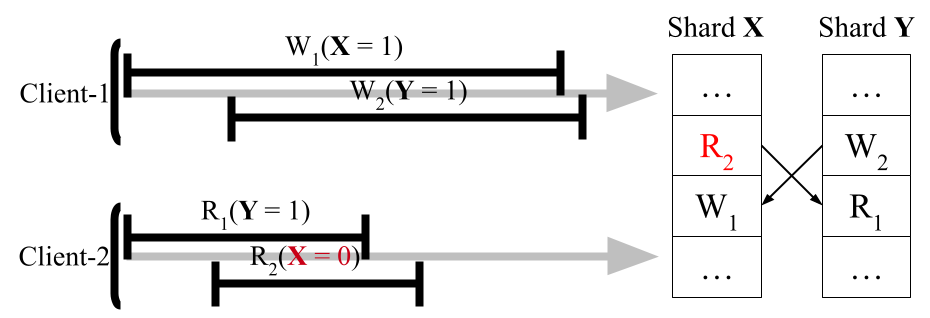
\includegraphics[scale=.45]{somet.png}
    \caption{Example execution where two concurrent clients each submit 2 concurrent requests. Assume keys \textbf{X} and \textbf{Y} are at different shards. It is possible that $R_2$ arrives before $W_1$ at shard \textbf{X}, and $W_2$ arrives before $R_1$ at shard \textbf{Y}. Since clients expect their concurrent requests to take affect in invocation order, if $R_1$ returns 1, then $W_1$ must have taken affect before $R_1$, so $R_2$ should necessarily return a value of 1.}
    \label{fig:concurrentbatches}
\end{figure}

For the single-shard setting, existing protocols come close to providing \MDL{}. A simple mechanism, such as per-client sequence numbers, can provide enough information for a shard leader to support invocation order for multiple requests from a single client. Such a solution does not suffice in the multi-shard setting, however, as shown in figure ~\ref{fig:concurrentbatches}. Linearizability is a local property, thus a single-shard protocol correctly scales to multiple shards. \MDL{}, however, is not a local property due to the possible interleaving of sets of concurrent requests across concurrent clients.
% Jeff: I don't think we want (or need) to make the claim below.
% This requires an \MDL{} protocol to use inter-shard communication in order to guarantee a safe total ordering that reflects issue order.

Sequence numbers are assigned at the client library 
and increase monotonically per shard. For example, a client issuing two requests for the first time to different keys that are on different shards will issue two requests both with sequence number 0. The shard leaders can then easily detect when a client's request
has arrived out of order and can buffer it until the necessary predecessor requests intended for the same shard arrive.
